\documentclass[a4paper,11pt,final]{article}
        \usepackage{fancyvrb, color, graphicx, hyperref, amsmath, url, textcomp}
        \usepackage{palatino}
        \usepackage[a4paper,text={16.5cm,25.2cm},centering]{geometry}

        %Set different options for xetex and luatex
        \usepackage{iftex}
        \ifxetex\usepackage{fontspec}\fi

        \ifluatex\usepackage{fontspec}\fi

        \usepackage{xcolor}
        % ANSI colors from nbconvert
        \definecolor{ansi-black}{HTML}{3E424D}
        \definecolor{ansi-black-intense}{HTML}{282C36}
        \definecolor{ansi-red}{HTML}{E75C58}
        \definecolor{ansi-red-intense}{HTML}{B22B31}
        \definecolor{ansi-green}{HTML}{00A250}
        \definecolor{ansi-green-intense}{HTML}{007427}
        \definecolor{ansi-yellow}{HTML}{DDB62B}
        \definecolor{ansi-yellow-intense}{HTML}{B27D12}
        \definecolor{ansi-blue}{HTML}{208FFB}
        \definecolor{ansi-blue-intense}{HTML}{0065CA}
        \definecolor{ansi-magenta}{HTML}{D160C4}
        \definecolor{ansi-magenta-intense}{HTML}{A03196}
        \definecolor{ansi-cyan}{HTML}{60C6C8}
        \definecolor{ansi-cyan-intense}{HTML}{258F8F}
        \definecolor{ansi-white}{HTML}{C5C1B4}
         \definecolor{ansi-white-intense}{HTML}{A1A6B2}

        \hypersetup
        {   pdfauthor = {Pweave},
            pdftitle={Published from FIR_designp.pmd},
            colorlinks=TRUE,
            linkcolor=black,
            citecolor=blue,
            urlcolor=blue
        }
        \setlength{\parindent}{0pt}
        \setlength{\parskip}{1.2ex}
        % fix for pandoc 1.14
        \providecommand{\tightlist}{%
            \setlength{\itemsep}{0pt}\setlength{\parskip}{0pt}}
        
\makeatletter
\def\PY@reset{\let\PY@it=\relax \let\PY@bf=\relax%
    \let\PY@ul=\relax \let\PY@tc=\relax%
    \let\PY@bc=\relax \let\PY@ff=\relax}
\def\PY@tok#1{\csname PY@tok@#1\endcsname}
\def\PY@toks#1+{\ifx\relax#1\empty\else%
    \PY@tok{#1}\expandafter\PY@toks\fi}
\def\PY@do#1{\PY@bc{\PY@tc{\PY@ul{%
    \PY@it{\PY@bf{\PY@ff{#1}}}}}}}
\def\PY#1#2{\PY@reset\PY@toks#1+\relax+\PY@do{#2}}

\@namedef{PY@tok@w}{\def\PY@tc##1{\textcolor[rgb]{0.73,0.73,0.73}{##1}}}
\@namedef{PY@tok@c}{\let\PY@it=\textit\def\PY@tc##1{\textcolor[rgb]{0.25,0.50,0.50}{##1}}}
\@namedef{PY@tok@cp}{\def\PY@tc##1{\textcolor[rgb]{0.74,0.48,0.00}{##1}}}
\@namedef{PY@tok@k}{\let\PY@bf=\textbf\def\PY@tc##1{\textcolor[rgb]{0.00,0.50,0.00}{##1}}}
\@namedef{PY@tok@kp}{\def\PY@tc##1{\textcolor[rgb]{0.00,0.50,0.00}{##1}}}
\@namedef{PY@tok@kt}{\def\PY@tc##1{\textcolor[rgb]{0.69,0.00,0.25}{##1}}}
\@namedef{PY@tok@o}{\def\PY@tc##1{\textcolor[rgb]{0.40,0.40,0.40}{##1}}}
\@namedef{PY@tok@ow}{\let\PY@bf=\textbf\def\PY@tc##1{\textcolor[rgb]{0.67,0.13,1.00}{##1}}}
\@namedef{PY@tok@nb}{\def\PY@tc##1{\textcolor[rgb]{0.00,0.50,0.00}{##1}}}
\@namedef{PY@tok@nf}{\def\PY@tc##1{\textcolor[rgb]{0.00,0.00,1.00}{##1}}}
\@namedef{PY@tok@nc}{\let\PY@bf=\textbf\def\PY@tc##1{\textcolor[rgb]{0.00,0.00,1.00}{##1}}}
\@namedef{PY@tok@nn}{\let\PY@bf=\textbf\def\PY@tc##1{\textcolor[rgb]{0.00,0.00,1.00}{##1}}}
\@namedef{PY@tok@ne}{\let\PY@bf=\textbf\def\PY@tc##1{\textcolor[rgb]{0.82,0.25,0.23}{##1}}}
\@namedef{PY@tok@nv}{\def\PY@tc##1{\textcolor[rgb]{0.10,0.09,0.49}{##1}}}
\@namedef{PY@tok@no}{\def\PY@tc##1{\textcolor[rgb]{0.53,0.00,0.00}{##1}}}
\@namedef{PY@tok@nl}{\def\PY@tc##1{\textcolor[rgb]{0.63,0.63,0.00}{##1}}}
\@namedef{PY@tok@ni}{\let\PY@bf=\textbf\def\PY@tc##1{\textcolor[rgb]{0.60,0.60,0.60}{##1}}}
\@namedef{PY@tok@na}{\def\PY@tc##1{\textcolor[rgb]{0.49,0.56,0.16}{##1}}}
\@namedef{PY@tok@nt}{\let\PY@bf=\textbf\def\PY@tc##1{\textcolor[rgb]{0.00,0.50,0.00}{##1}}}
\@namedef{PY@tok@nd}{\def\PY@tc##1{\textcolor[rgb]{0.67,0.13,1.00}{##1}}}
\@namedef{PY@tok@s}{\def\PY@tc##1{\textcolor[rgb]{0.73,0.13,0.13}{##1}}}
\@namedef{PY@tok@sd}{\let\PY@it=\textit\def\PY@tc##1{\textcolor[rgb]{0.73,0.13,0.13}{##1}}}
\@namedef{PY@tok@si}{\let\PY@bf=\textbf\def\PY@tc##1{\textcolor[rgb]{0.73,0.40,0.53}{##1}}}
\@namedef{PY@tok@se}{\let\PY@bf=\textbf\def\PY@tc##1{\textcolor[rgb]{0.73,0.40,0.13}{##1}}}
\@namedef{PY@tok@sr}{\def\PY@tc##1{\textcolor[rgb]{0.73,0.40,0.53}{##1}}}
\@namedef{PY@tok@ss}{\def\PY@tc##1{\textcolor[rgb]{0.10,0.09,0.49}{##1}}}
\@namedef{PY@tok@sx}{\def\PY@tc##1{\textcolor[rgb]{0.00,0.50,0.00}{##1}}}
\@namedef{PY@tok@m}{\def\PY@tc##1{\textcolor[rgb]{0.40,0.40,0.40}{##1}}}
\@namedef{PY@tok@gh}{\let\PY@bf=\textbf\def\PY@tc##1{\textcolor[rgb]{0.00,0.00,0.50}{##1}}}
\@namedef{PY@tok@gu}{\let\PY@bf=\textbf\def\PY@tc##1{\textcolor[rgb]{0.50,0.00,0.50}{##1}}}
\@namedef{PY@tok@gd}{\def\PY@tc##1{\textcolor[rgb]{0.63,0.00,0.00}{##1}}}
\@namedef{PY@tok@gi}{\def\PY@tc##1{\textcolor[rgb]{0.00,0.63,0.00}{##1}}}
\@namedef{PY@tok@gr}{\def\PY@tc##1{\textcolor[rgb]{1.00,0.00,0.00}{##1}}}
\@namedef{PY@tok@ge}{\let\PY@it=\textit}
\@namedef{PY@tok@gs}{\let\PY@bf=\textbf}
\@namedef{PY@tok@gp}{\let\PY@bf=\textbf\def\PY@tc##1{\textcolor[rgb]{0.00,0.00,0.50}{##1}}}
\@namedef{PY@tok@go}{\def\PY@tc##1{\textcolor[rgb]{0.53,0.53,0.53}{##1}}}
\@namedef{PY@tok@gt}{\def\PY@tc##1{\textcolor[rgb]{0.00,0.27,0.87}{##1}}}
\@namedef{PY@tok@err}{\def\PY@bc##1{{\setlength{\fboxsep}{\string -\fboxrule}\fcolorbox[rgb]{1.00,0.00,0.00}{1,1,1}{\strut ##1}}}}
\@namedef{PY@tok@kc}{\let\PY@bf=\textbf\def\PY@tc##1{\textcolor[rgb]{0.00,0.50,0.00}{##1}}}
\@namedef{PY@tok@kd}{\let\PY@bf=\textbf\def\PY@tc##1{\textcolor[rgb]{0.00,0.50,0.00}{##1}}}
\@namedef{PY@tok@kn}{\let\PY@bf=\textbf\def\PY@tc##1{\textcolor[rgb]{0.00,0.50,0.00}{##1}}}
\@namedef{PY@tok@kr}{\let\PY@bf=\textbf\def\PY@tc##1{\textcolor[rgb]{0.00,0.50,0.00}{##1}}}
\@namedef{PY@tok@bp}{\def\PY@tc##1{\textcolor[rgb]{0.00,0.50,0.00}{##1}}}
\@namedef{PY@tok@fm}{\def\PY@tc##1{\textcolor[rgb]{0.00,0.00,1.00}{##1}}}
\@namedef{PY@tok@vc}{\def\PY@tc##1{\textcolor[rgb]{0.10,0.09,0.49}{##1}}}
\@namedef{PY@tok@vg}{\def\PY@tc##1{\textcolor[rgb]{0.10,0.09,0.49}{##1}}}
\@namedef{PY@tok@vi}{\def\PY@tc##1{\textcolor[rgb]{0.10,0.09,0.49}{##1}}}
\@namedef{PY@tok@vm}{\def\PY@tc##1{\textcolor[rgb]{0.10,0.09,0.49}{##1}}}
\@namedef{PY@tok@sa}{\def\PY@tc##1{\textcolor[rgb]{0.73,0.13,0.13}{##1}}}
\@namedef{PY@tok@sb}{\def\PY@tc##1{\textcolor[rgb]{0.73,0.13,0.13}{##1}}}
\@namedef{PY@tok@sc}{\def\PY@tc##1{\textcolor[rgb]{0.73,0.13,0.13}{##1}}}
\@namedef{PY@tok@dl}{\def\PY@tc##1{\textcolor[rgb]{0.73,0.13,0.13}{##1}}}
\@namedef{PY@tok@s2}{\def\PY@tc##1{\textcolor[rgb]{0.73,0.13,0.13}{##1}}}
\@namedef{PY@tok@sh}{\def\PY@tc##1{\textcolor[rgb]{0.73,0.13,0.13}{##1}}}
\@namedef{PY@tok@s1}{\def\PY@tc##1{\textcolor[rgb]{0.73,0.13,0.13}{##1}}}
\@namedef{PY@tok@mb}{\def\PY@tc##1{\textcolor[rgb]{0.40,0.40,0.40}{##1}}}
\@namedef{PY@tok@mf}{\def\PY@tc##1{\textcolor[rgb]{0.40,0.40,0.40}{##1}}}
\@namedef{PY@tok@mh}{\def\PY@tc##1{\textcolor[rgb]{0.40,0.40,0.40}{##1}}}
\@namedef{PY@tok@mi}{\def\PY@tc##1{\textcolor[rgb]{0.40,0.40,0.40}{##1}}}
\@namedef{PY@tok@il}{\def\PY@tc##1{\textcolor[rgb]{0.40,0.40,0.40}{##1}}}
\@namedef{PY@tok@mo}{\def\PY@tc##1{\textcolor[rgb]{0.40,0.40,0.40}{##1}}}
\@namedef{PY@tok@ch}{\let\PY@it=\textit\def\PY@tc##1{\textcolor[rgb]{0.25,0.50,0.50}{##1}}}
\@namedef{PY@tok@cm}{\let\PY@it=\textit\def\PY@tc##1{\textcolor[rgb]{0.25,0.50,0.50}{##1}}}
\@namedef{PY@tok@cpf}{\let\PY@it=\textit\def\PY@tc##1{\textcolor[rgb]{0.25,0.50,0.50}{##1}}}
\@namedef{PY@tok@c1}{\let\PY@it=\textit\def\PY@tc##1{\textcolor[rgb]{0.25,0.50,0.50}{##1}}}
\@namedef{PY@tok@cs}{\let\PY@it=\textit\def\PY@tc##1{\textcolor[rgb]{0.25,0.50,0.50}{##1}}}

\def\PYZbs{\char`\\}
\def\PYZus{\char`\_}
\def\PYZob{\char`\{}
\def\PYZcb{\char`\}}
\def\PYZca{\char`\^}
\def\PYZam{\char`\&}
\def\PYZlt{\char`\<}
\def\PYZgt{\char`\>}
\def\PYZsh{\char`\#}
\def\PYZpc{\char`\%}
\def\PYZdl{\char`\$}
\def\PYZhy{\char`\-}
\def\PYZsq{\char`\'}
\def\PYZdq{\char`\"}
\def\PYZti{\char`\~}
% for compatibility with earlier versions
\def\PYZat{@}
\def\PYZlb{[}
\def\PYZrb{]}
\makeatother

        
\title{ FIR filter design with Python and SciPy}
\author{ Matti Pastell}
\date{ 15th April 2013}

\begin{document}
\maketitle


\begin{Verbatim}[commandchars=\\\{\},frame=single,fontsize=\small, xleftmargin=0.5em]
\PY{k+kn}{from} \PY{n+nn}{pylab} \PY{k+kn}{import} \PY{o}{*}
\PY{k+kn}{import} \PY{n+nn}{scipy}\PY{n+nn}{.}\PY{n+nn}{signal} \PY{k}{as} \PY{n+nn}{signal}

\PY{c+c1}{\PYZsh{}Plot frequency and phase response}
\PY{k}{def} \PY{n+nf}{mfreqz}\PY{p}{(}\PY{n}{b}\PY{p}{,}\PY{n}{a}\PY{o}{=}\PY{l+m+mi}{1}\PY{p}{)}\PY{p}{:}
    \PY{n}{w}\PY{p}{,}\PY{n}{h} \PY{o}{=} \PY{n}{signal}\PY{o}{.}\PY{n}{freqz}\PY{p}{(}\PY{n}{b}\PY{p}{,}\PY{n}{a}\PY{p}{)}
    \PY{n}{h\PYZus{}dB} \PY{o}{=} \PY{l+m+mi}{20} \PY{o}{*} \PY{n}{log10} \PY{p}{(}\PY{n+nb}{abs}\PY{p}{(}\PY{n}{h}\PY{p}{)}\PY{p}{)}
    \PY{n}{subplot}\PY{p}{(}\PY{l+m+mi}{211}\PY{p}{)}
    \PY{n}{plot}\PY{p}{(}\PY{n}{w}\PY{o}{/}\PY{n+nb}{max}\PY{p}{(}\PY{n}{w}\PY{p}{)}\PY{p}{,}\PY{n}{h\PYZus{}dB}\PY{p}{)}
    \PY{n}{ylim}\PY{p}{(}\PY{o}{\PYZhy{}}\PY{l+m+mi}{150}\PY{p}{,} \PY{l+m+mi}{5}\PY{p}{)}
    \PY{n}{ylabel}\PY{p}{(}\PY{l+s+s1}{\PYZsq{}}\PY{l+s+s1}{Magnitude (db)}\PY{l+s+s1}{\PYZsq{}}\PY{p}{)}
    \PY{n}{xlabel}\PY{p}{(}\PY{l+s+sa}{r}\PY{l+s+s1}{\PYZsq{}}\PY{l+s+s1}{Normalized Frequency (x\PYZdl{}}\PY{l+s+s1}{\PYZbs{}}\PY{l+s+s1}{pi\PYZdl{}rad/sample)}\PY{l+s+s1}{\PYZsq{}}\PY{p}{)}
    \PY{n}{title}\PY{p}{(}\PY{l+s+sa}{r}\PY{l+s+s1}{\PYZsq{}}\PY{l+s+s1}{Frequency response}\PY{l+s+s1}{\PYZsq{}}\PY{p}{)}
    \PY{n}{subplot}\PY{p}{(}\PY{l+m+mi}{212}\PY{p}{)}
    \PY{n}{h\PYZus{}Phase} \PY{o}{=} \PY{n}{unwrap}\PY{p}{(}\PY{n}{arctan2}\PY{p}{(}\PY{n}{imag}\PY{p}{(}\PY{n}{h}\PY{p}{)}\PY{p}{,}\PY{n}{real}\PY{p}{(}\PY{n}{h}\PY{p}{)}\PY{p}{)}\PY{p}{)}
    \PY{n}{plot}\PY{p}{(}\PY{n}{w}\PY{o}{/}\PY{n+nb}{max}\PY{p}{(}\PY{n}{w}\PY{p}{)}\PY{p}{,}\PY{n}{h\PYZus{}Phase}\PY{p}{)}
    \PY{n}{ylabel}\PY{p}{(}\PY{l+s+s1}{\PYZsq{}}\PY{l+s+s1}{Phase (radians)}\PY{l+s+s1}{\PYZsq{}}\PY{p}{)}
    \PY{n}{xlabel}\PY{p}{(}\PY{l+s+sa}{r}\PY{l+s+s1}{\PYZsq{}}\PY{l+s+s1}{Normalized Frequency (x\PYZdl{}}\PY{l+s+s1}{\PYZbs{}}\PY{l+s+s1}{pi\PYZdl{}rad/sample)}\PY{l+s+s1}{\PYZsq{}}\PY{p}{)}
    \PY{n}{title}\PY{p}{(}\PY{l+s+sa}{r}\PY{l+s+s1}{\PYZsq{}}\PY{l+s+s1}{Phase response}\PY{l+s+s1}{\PYZsq{}}\PY{p}{)}
    \PY{n}{\PYZus{}} \PY{o}{=} \PY{n}{subplots\PYZus{}adjust}\PY{p}{(}\PY{n}{hspace}\PY{o}{=}\PY{l+m+mi}{1}\PY{p}{)}
    \PY{n}{show}\PY{p}{(}\PY{p}{)}

\PY{c+c1}{\PYZsh{}Plot step and impulse response}
\PY{k}{def} \PY{n+nf}{impz}\PY{p}{(}\PY{n}{b}\PY{p}{,}\PY{n}{a}\PY{o}{=}\PY{l+m+mi}{1}\PY{p}{)}\PY{p}{:}
    \PY{n}{l} \PY{o}{=} \PY{n+nb}{len}\PY{p}{(}\PY{n}{b}\PY{p}{)}
    \PY{n}{impulse} \PY{o}{=} \PY{n}{repeat}\PY{p}{(}\PY{l+m+mf}{0.}\PY{p}{,}\PY{n}{l}\PY{p}{)}\PY{p}{;} \PY{n}{impulse}\PY{p}{[}\PY{l+m+mi}{0}\PY{p}{]} \PY{o}{=}\PY{l+m+mf}{1.}
    \PY{n}{x} \PY{o}{=} \PY{n}{arange}\PY{p}{(}\PY{l+m+mi}{0}\PY{p}{,}\PY{n}{l}\PY{p}{)}
    \PY{n}{response} \PY{o}{=} \PY{n}{signal}\PY{o}{.}\PY{n}{lfilter}\PY{p}{(}\PY{n}{b}\PY{p}{,}\PY{n}{a}\PY{p}{,}\PY{n}{impulse}\PY{p}{)}
    \PY{n}{subplot}\PY{p}{(}\PY{l+m+mi}{211}\PY{p}{)}
    \PY{n}{stem}\PY{p}{(}\PY{n}{x}\PY{p}{,} \PY{n}{response}\PY{p}{)}
    \PY{n}{ylabel}\PY{p}{(}\PY{l+s+s1}{\PYZsq{}}\PY{l+s+s1}{Amplitude}\PY{l+s+s1}{\PYZsq{}}\PY{p}{)}
    \PY{n}{xlabel}\PY{p}{(}\PY{l+s+sa}{r}\PY{l+s+s1}{\PYZsq{}}\PY{l+s+s1}{n (samples)}\PY{l+s+s1}{\PYZsq{}}\PY{p}{)}
    \PY{n}{title}\PY{p}{(}\PY{l+s+sa}{r}\PY{l+s+s1}{\PYZsq{}}\PY{l+s+s1}{Impulse response}\PY{l+s+s1}{\PYZsq{}}\PY{p}{)}
    \PY{n}{subplot}\PY{p}{(}\PY{l+m+mi}{212}\PY{p}{)}
    \PY{n}{step} \PY{o}{=} \PY{n}{cumsum}\PY{p}{(}\PY{n}{response}\PY{p}{)}
    \PY{n}{stem}\PY{p}{(}\PY{n}{x}\PY{p}{,} \PY{n}{step}\PY{p}{)}
    \PY{n}{ylabel}\PY{p}{(}\PY{l+s+s1}{\PYZsq{}}\PY{l+s+s1}{Amplitude}\PY{l+s+s1}{\PYZsq{}}\PY{p}{)}
    \PY{n}{xlabel}\PY{p}{(}\PY{l+s+sa}{r}\PY{l+s+s1}{\PYZsq{}}\PY{l+s+s1}{n (samples)}\PY{l+s+s1}{\PYZsq{}}\PY{p}{)}
    \PY{n}{title}\PY{p}{(}\PY{l+s+sa}{r}\PY{l+s+s1}{\PYZsq{}}\PY{l+s+s1}{Step response}\PY{l+s+s1}{\PYZsq{}}\PY{p}{)}
    \PY{n}{\PYZus{}} \PY{o}{=} \PY{n}{subplots\PYZus{}adjust}\PY{p}{(}\PY{n}{hspace}\PY{o}{=}\PY{l+m+mi}{1}\PY{p}{)}
    \PY{n}{show}\PY{p}{(}\PY{p}{)}
\end{Verbatim}



\begin{Verbatim}[commandchars=\\\{\},frame=single,fontsize=\small, xleftmargin=0.5em]
\PY{n}{n} \PY{o}{=} \PY{l+m+mi}{61}
\PY{n}{a} \PY{o}{=} \PY{n}{signal}\PY{o}{.}\PY{n}{firwin}\PY{p}{(}\PY{n}{n}\PY{p}{,} \PY{n}{cutoff} \PY{o}{=} \PY{l+m+mf}{0.3}\PY{p}{,} \PY{n}{window} \PY{o}{=} \PY{l+s+s2}{\PYZdq{}}\PY{l+s+s2}{hamming}\PY{l+s+s2}{\PYZdq{}}\PY{p}{)}
\PY{c+c1}{\PYZsh{}Frequency and phase response}
\PY{n}{mfreqz}\PY{p}{(}\PY{n}{a}\PY{p}{)}
\end{Verbatim}
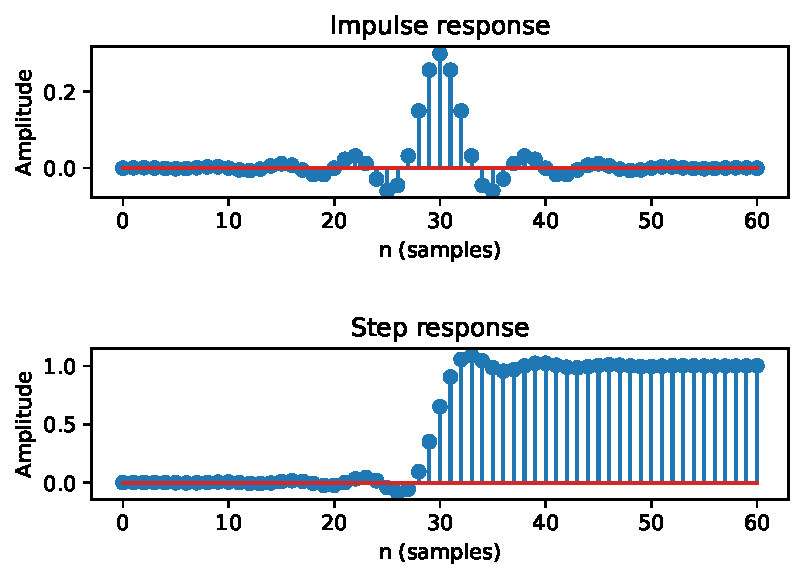
\includegraphics[width= \linewidth]{figures/FIR_designp_figure2_1.pdf}


\begin{Verbatim}[commandchars=\\\{\},frame=single,fontsize=\small, xleftmargin=0.5em]
\PY{c+c1}{\PYZsh{}Impulse and step response}
\PY{n}{impz}\PY{p}{(}\PY{n}{a}\PY{p}{)}
\end{Verbatim}
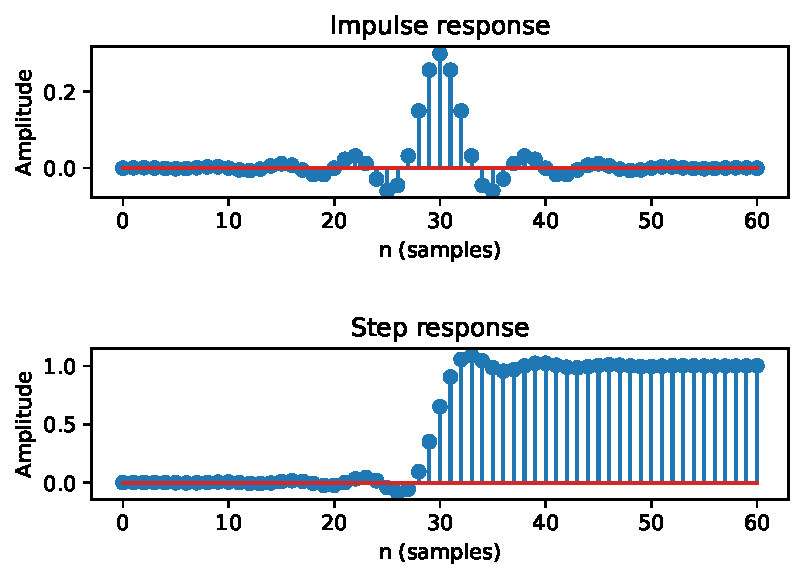
\includegraphics[width= \linewidth]{figures/FIR_designp_figure2_1.pdf}



\begin{Verbatim}[commandchars=\\\{\},frame=single,fontsize=\small, xleftmargin=0.5em]
\PY{n}{n} \PY{o}{=} \PY{l+m+mi}{101}
\PY{n}{a} \PY{o}{=} \PY{n}{signal}\PY{o}{.}\PY{n}{firwin}\PY{p}{(}\PY{n}{n}\PY{p}{,} \PY{n}{cutoff} \PY{o}{=} \PY{l+m+mf}{0.3}\PY{p}{,} \PY{n}{window} \PY{o}{=} \PY{l+s+s2}{\PYZdq{}}\PY{l+s+s2}{hanning}\PY{l+s+s2}{\PYZdq{}}\PY{p}{,} \PY{n}{pass\PYZus{}zero}\PY{o}{=}\PY{k+kc}{False}\PY{p}{)}
\PY{n}{mfreqz}\PY{p}{(}\PY{n}{a}\PY{p}{)}
\end{Verbatim}
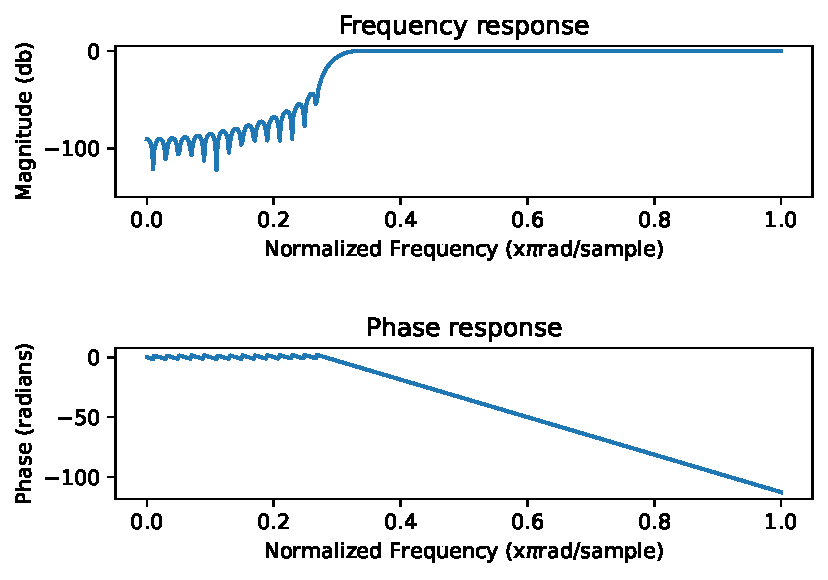
\includegraphics[width= \linewidth]{figures/FIR_designp_figure3_1.pdf}



\begin{Verbatim}[commandchars=\\\{\},frame=single,fontsize=\small, xleftmargin=0.5em]
\PY{n}{n} \PY{o}{=} \PY{l+m+mi}{1001}
\PY{n}{a} \PY{o}{=} \PY{n}{signal}\PY{o}{.}\PY{n}{firwin}\PY{p}{(}\PY{n}{n}\PY{p}{,} \PY{n}{cutoff} \PY{o}{=} \PY{p}{[}\PY{l+m+mf}{0.2}\PY{p}{,} \PY{l+m+mf}{0.5}\PY{p}{]}\PY{p}{,} \PY{n}{window} \PY{o}{=} \PY{l+s+s1}{\PYZsq{}}\PY{l+s+s1}{blackmanharris}\PY{l+s+s1}{\PYZsq{}}\PY{p}{,} \PY{n}{pass\PYZus{}zero} \PY{o}{=} \PY{k+kc}{False}\PY{p}{)}
\PY{n}{mfreqz}\PY{p}{(}\PY{n}{a}\PY{p}{)}
\end{Verbatim}
\begin{figure}[htpb]
\center
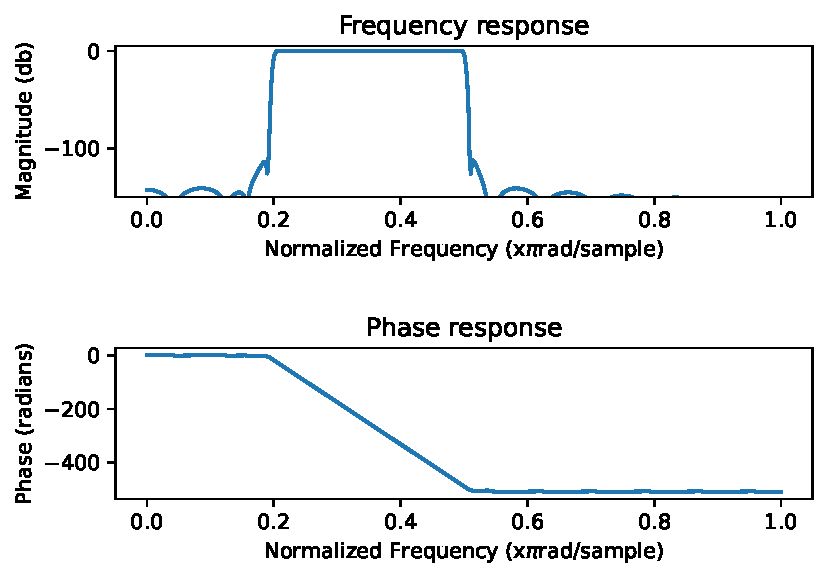
\includegraphics[width= \linewidth]{figures/FIR_designp_figure4_1.pdf}
\caption{Bandpass FIR filter.}
\label{fig:None}
\end{figure}

\end{document}